\documentclass[prodmode,acmtoplas]{acmsmall} % Aptara syntax

% Package to generate and customize Algorithm as per ACM style
\usepackage[ruled]{algorithm2e}
\renewcommand{\algorithmcfname}{ALGORITHM}
\SetAlFnt{\small}
\SetAlCapFnt{\small}
\SetAlCapNameFnt{\small}
\SetAlCapHSkip{0pt}
\IncMargin{-\parindent}

% Metadata Information
\acmVolume{9}
\acmNumber{4}
\acmArticle{39}
\acmYear{2010}
\acmMonth{3}

% Copyright
%\setcopyright{acmcopyright}
%\setcopyright{acmlicensed}
%\setcopyright{rightsretained}
%\setcopyright{usgov}
%\setcopyright{usgovmixed}
%\setcopyright{cagov}
%\setcopyright{cagovmixed}

% DOI
\doi{0000001.0000001}

%ISSN
\issn{1234-56789}


\usepackage{amsmath}
%\usepackage{amssymb}
%\usepackage{amsthm}

\usepackage{multicol}
\usepackage{multirow}
\usepackage{graphicx}
\usepackage{color}
\usepackage{subfigure}
\usepackage{epsfig}
\usepackage{fancybox}
\usepackage{fancyvrb}

\usepackage{array}
\usepackage{mdwmath}
\usepackage{mdwtab}
\usepackage{eqparbox}

% CHR
\usepackage[T1]{fontenc}
\usepackage[latin9]{inputenc}
\usepackage{units}
%\usepackage{amsmath}
\usepackage{stackrel}
%\usepackage{esint}
%\usepackage{babel}



%\usepackage{amssymb}
%\usepackage{amsthm}

\usepackage{hyperref} % comes last, as it redefines a couple of commands
\hypersetup{
    colorlinks,%
    citecolor=black,%
    filecolor=black,%
    linkcolor=black,%
    urlcolor=blue
}

\DefineVerbatimEnvironment{colorcode}%
        {Verbatim}{fontsize=\scriptsize,commandchars=\\\{\}}


\definecolor{Red}{RGB}{220,50,10}
\definecolor{Blue}{RGB}{0,51,102}
\definecolor{Yellow}{RGB}{102,51,0}
\definecolor{Orange}{RGB}{178,36,36}
\definecolor{Grey}{RGB}{180,180,180}
\definecolor{Green}{RGB}{20,120,20}
\definecolor{Purple}{RGB}{160,50,100}
\newcommand{\red}[1]{\textcolor{Red}{{#1}}}
\newcommand{\blue}[1]{\textcolor{Blue}{{#1}}}
\newcommand{\yellow}[1]{\textcolor{Yellow}{{#1}}}
\newcommand{\orange}[1]{\textcolor{Orange}{{#1}}}
\newcommand{\grey}[1]{\textcolor{Grey}{{#1}}}
\newcommand{\green}[1]{\textcolor{Green}{{#1}}}
\newcommand{\purple}[1]{\textcolor{Purple}{{#1}}}


\definecolor{DikuRed}{RGB}{130,50,32}
\newcommand{\emp}[1]{\textcolor{DikuRed}{ #1}}
\definecolor{CosGreen}{RGB}{10,100,70}
\newcommand{\emphh}[1]{\textcolor{CosGreen}{ #1}}


\newcommand{\mymath}[1]{$ #1 $}
\newcommand{\myindx}[1]{_{#1}}
\newcommand{\myindu}[1]{^{#1}}
\newcommand{\mymathbb}[1]{\mathbb{#1}}

\newcommand{\memo}[1]{\noindent \textbf{MEMO: #1}}
\newcommand{\bra}[1]{\texttt{\{}#1\texttt{\}}}
\newcommand{\para}[1]{\texttt{(} #1 \texttt{)}}

% Document starts
\begin{document}

% Page heads
\markboth{C. Oancea and L. Rauchwerger}{Predicate-Based Hybrid Analysis}

% Title portion
\title{Predicate-Based Hybrid Analysis}
\author{Cosmin E. Oancea and Lawrence Rauchwerger
\affil{Texas A\&M University}
%Lawrence Rauchwerger
%\affil{Texas A\&M University}
}

\begin{abstract}
%%%%%%%%%%%%%%%%%%%%%%%%%%%%%%%%%%%%%%%%%%%%%%%%%%%%%%%%
%%% What are we doing here?
%%% Framework for hybrid analysis pertaining 
%%% memory-reference analysis for:
%%% 1. autoparallelization, 2. array SSA,
%%% 3. optimization of copy in/out, 4. size analysis
%%%%%%%%%%%%%%%%%%%%%%%%%%%%%%%%%%%%%%%%%%%%%%%%%%%%%%%%
This paper presents a framework for memory-reference analysis that
integrates the use of static and run-time (hybrid) techniques
to overcome many of the known difficulties arising in such a context,
i.e., it solves large loops with complex control flow that use various 
kinds of non-affine subscripts, such as indirect arrays, quadratic loop indices
or induction variables that cannot be expressed as a closed-form formula in 
the enclosing loop-nest indices ({\sc civ}).
%
Our framework is primarily demonstrated by automatically proving the 
parallelism of {\tt Fortran77} loops, i.e., dependence analysis, 
but has other applications such as
(i)   optimizing the copying between global and private memory,
(ii)  size analysis and %, e.g., for optimized reduction.
(iii) array {\sc ssa}~\cite{arraySSA}.


%%%%%%%%%%%%%%%%%%%%%%%%%%%%%%%%%%%%%%%%%%%%%%%%%%%%%%%%
%%% How are we doing it?
%%% 1. accurate prg-level rep of array references with 
%%%    abstract sets @ every level in the program via
%%%    data-flow analysis.
%%% 2. @loop level: build ``dependence summary'' D, as 
%%%    compact as possible from the computed abstract 
%%%    sets, such as D accurately describes the memory 
%%%    references involved in dependences.
%%% 3. our rep is good enough to give:
%%%    (i)  doall parallelism (D=\emptyset), 
%%%    (ii) privatisation and (iii) reduction.
%%%%%%%%%%%%%%%%%%%%%%%%%%%%%%%%%%%%%%%%%%%%%%%%%%%%%%%%
Our approach builds on a data-flow technique that accurately represents/summarizes
array references as abstract sets at every level in the program.
%
At this stage we proposed several improvements to the base analysis,
notably a technique that produces more compact and effective abstract sets
for {\sc civ}-based subscripts.
%and more likely to succeed representation for {\sc civ}-based subscripts.
%
Then, at every loop level, a ``dependence summary'' $D$ is constructed 
from the computed abstract sets, such that $D$ accurately describes the memory 
references involved in cross-iteration dependencies.

This representation is good enough to model do-all parallelism, 
privatization and reduction (and can act as a filter if 
direction vectors are required).
%are required, i.e., the precise pair of program points involved in a dependency. 
%
%%%%%%%%%%%%%%%%%%%%%%%%%%%%%%%%%%%%%%%%%%%%%%%%%%%%%%%%%%%%%%%%%%%%
%%% 4. In difficult cases D cannot be evaluated 
%%%    symbolically and direct runtime evaluation will
%%%    introduce significant overhead. Instead we continue
%%%    static analysis by translating D to a predicate that
%%%    can be further simplified statically and introduces
%%%    negligible overhead. Achieved by factoring sufficient
%%%    conditions of D = \emptyset equation.
%%%%%%%%%%%%%%%%%%%%%%%%%%%%%%%%%%%%%%%%%%%%%%%%%%%%%%%%%%%%%%%%%%%%
In difficult cases however, $D$ cannot be evaluated symbolically and its
runtime evaluation would introduce significant overhead. %, if not prohibitive overhead. 
%
Instead, we continue static analysis by translating $D$ into a predicate $P$
by factoring out the sufficient conditions of equation $D = \emptyset$. 

The summary-to-predicate translation relies on a set of (easily extensible) 
logical-inference rules that range from simple, e.g., a sufficient condition 
for $A\cap B=\emptyset$ is $A = \emptyset$, to complex rules that exploit the 
assumed (and statically verified) monotonicity of the sub-terms of an irreducible 
recurrence. 
%
The proposed technique introduces in practice negligible overhead, 
because $P$ can be further simplified statically, for example by separating 
it into a sequence of predicates $P=P_1\vee\ldots\vee P_n$ of increasing 
runtime complexities, which, if statically irreducible, are evaluated in 
order until one succeeds or all fail.

We evaluate our automated solution on about $30$ benchmarks, including
{\sc perfect-club} and {\sc spec} suites, and show that our approach
is effective in parallelizing large, complex loops and obtains much better 
full program speedups than the Intel and IBM Fortran compilers.
%
While other related work also uses deferred analysis, our approach is unique 
in that it translates the problem entirely to the logical realm, and solves 
uniformly a set of difficult loops that were either not reported before or 
were solved with different techniques.
\end{abstract}

\begin{CCSXML}
<ccs2012>
<concept>
<concept_id>10011007.10011006.10011041</concept_id>
<concept_desc>Software and its engineering~Compilers</concept_desc>
<concept_significance>500</concept_significance>
</concept>
<concept>
<concept_id>10010147.10010169.10010175</concept_id>
<concept_desc>Computing methodologies~Parallel programming languages</concept_desc>
<concept_significance>500</concept_significance>
</concept>
</ccs2012>
\end{CCSXML}

\ccsdesc[500]{Computing methodologies~Parallel programming languages}
\ccsdesc[500]{Software and its engineering~Compilers}

%
% End generated code
%

% We no longer use \terms command
%\terms{Design, Algorithms, Performance}

\keywords{automatic parallelization, summarization, privatization, reduction.}
%, Fortran do loops

\acmformat{Cosmin Oancea and Lawrence Rauchwerger, 2015. Predicate-Based Hybrid Analysis.}
% At a minimum you need to supply the author names, year and a title.
% IMPORTANT:
% Full first names whenever they are known, surname last, followed by a period.
% In the case of two authors, 'and' is placed between them.
% In the case of three or more authors, the serial comma is used, that is, all author names
% except the last one but including the penultimate author's name are followed by a comma,
% and then 'and' is placed before the final author's name.
% If only first and middle initials are known, then each initial
% is followed by a period and they are separated by a space.
% The remaining information (journal title, volume, article number, date, etc.) is 'auto-generated'.

\begin{bottomstuff}
This work was supported in part by NSF awards CRI-0551685, CCF-0833199, CCF-0830753, 
IIS-0917266, NSF/DNDO award 2008-DN-077-ARI018-02, by the DOE NNSA PSAAP  grant 
DE-FC52-08NA28616, IBM, Intel, Oracle/Sun and Award KUS-C1-016-04, made by King Abdullah
University of Science and Technology (KAUST), and by Danish Strategic Research Council,
for the HIPERFIT research center under contract 10-092299.

Author's addresses: 
Cosmin E. Oancea, Hiperfit, Computer Science Department, (DIKU), University of Copenhagen; 
Lawrence Rauchwerger, Parasol Lab, Department of Computer Science and Engineering, Texas A\&M University.
\end{bottomstuff}

\maketitle

\section{Introduction}



%%%%%%%%%%%%%%%%%%%%%%%%%%%%%%%%%%%%%%%%%
%%% INTRODUCTION: RUN TIME TECHNIQUES %%%
%%%%%%%%%%%%%%%%%%%%%%%%%%%%%%%%%%%%%%%%%

Automatic loop parallelization requires the analysis of  memory 
references for the purpose of establishing their data independence.
For array references, compilers have used data dependence analysis
which has historically taken two distinct directions:
Static (compile time) analysis and run-time (dynamic) analysis. 

%%%%%%%%%%%%%%%%%%%%%%%%%%%%%%%%%%%%%%%%%%%%%%%%%%%%%%%%%%
%%%  INTRODUCTION: SHORT HISTORY OF STATIC TECHNIQUES  %%%
%%%%%%%%%%%%%%%%%%%%%%%%%%%%%%%%%%%%%%%%%%%%%%%%%%%%%%%%%%

{\em Static dependence analysis}, first proposed by 
~\cite{OptCompModernArch,BanerjeeIneqTest,FeautrierDataflow,Pugh92theomega}, 
analyzes an entire loop nest by modeling the data dependencies 
between any pair of read/write accesses. While this technique 
can also drive powerful code 
transformations such as loop interchange, skewing, etc.,
they are typically limited to the affine array subscript domain and
their effectiveness~\cite{PolyhedralOpt} is limited to relatively-small loop nests.
However, in the more general case, there are many obstacles 
to loop parallelization such as difficult to analyze 
symbolic constants, complex control flow, array-reshaping at call sites, 
quadratic array indexing, induction variables with no closed-form solutions
~\cite{Blume92PerfectCodesEval,LMAD,SUIF}.
Various techniques have been proposed to partially address some of these
difficulties. For example, a class of index-array and stack-like accesses may
be disambiguated via access pattern-matching 
techniques~\cite{PaduaStackArr,PaduaDemDrInterproc}
and some monotonic accesses (e.g., quadratic indexing) can be 
disambiguated via non-affine dependency tests~\cite{Blume94RangeTest}.
Similarly, Presburger arithmetic
can be extended to the non-affine domain~\cite{Pugh98NonlinPresb} to solve a 
class of irregular accesses and control-flow.
%
The next step has been to extend analysis to program level by summarizing accesses
interprocedurally, where an array abstraction is used to represent a (regular) set 
of memory references either via  systems of affine constraints~\cite{SUIF}, 
or linear-memory-access descriptors~\cite{LMAD}, respectively.
%
Loop independence has been modeled typically via an equation on summaries of 
shape $S=\emptyset$. To improve precision, summaries are paired with 
predicates~\cite{Moon99PredArrDataFlow,HoeflingerDepTest}
that guard (otherwise unsafe) simplifications in the array-abstraction domain or 
predicate the summary existence (i.e., control-flow conditions).
%

{\em Run-time analysis} is necessary and useful  when static analysis alone 
cannot decide whether a loop is independent or not and thus needs to make the 
conservative choice, i.e., not parallel.  Run-time analysis can always resolve
static ambiguities because it can use instances of symbols and thus produce accurate 
results. Historically,  dynamic  dependence analysis has been performed by 
tracing and analyzing a loop's relevant memory references 
by executing an inspector loop (inspector/executor 
model~\cite{InspExecWave}), or by tracing and analyzing 
a speculative parallel execution of the loop
as it is done in thread-level speculation~\cite{LRPD}.   
Such approaches typically extract maximal parallelism, at the cost
of  significant overhead, usually  proportional to the number of 
traced dynamic memory references. 

In order to  attain our goal of effectively parallelizing
a large number of codes automatically we have devised a hybrid compiler technology 
that can extract maximum static information so that the overhead of the 
dynamic analysis is reduced to a minimum.

\subsection{Static Analysis with Light Weight Dynamic Complement }
\label{subsec:ProposedSolHL}

Summary based static analysis based on the array abstraction has been shown 
by previous research to be more scalable and useful for loop parallelization. 
However,  from our experience we have found that its main source of inaccuracy 
lies in the fact that the array abstraction does not form a closed algebra 
under the required 
set operations: (recurrence) union, intersection, subtraction, gates, 
call sites. This shortcoming results in the necessity of conservative approximations 
during early 
construction stages, both at the array-abstraction and its associated-predicate 
levels. Thus either fewer loops are qualified as parallel or more dynamic analysis is 
needed.
To mitigate this lack of scalability we have adopted a more expressive,
higher level intermediate representation language. 
We are using the {\sc usr}(Uniform Set Representation)~\cite{HybAn},
  a composable language that subsumes both the array abstraction 
as well as the control flow. It includes in the language results of operations
previously deemed outside the array-abstraction  domain.
Thus we can express the  loop data independence summary equation 
as a the set equation  $S = \emptyset$. Sometimes this equation is easy to prove 
statically. However,  usually for real codes,
the {\sc usr} which needs to be proven empty is very complex. Furthermore, for outer 
loops, the set expressions become very long and cumbersome to deal with 
during compilation. 

To deal with this problem in a scalable manner, i.e., for outer, program level 
loops, we define an equally-rich  language of predicates ({\sc pdag}) and 
an 
effective rule-based translation between the two languages, such that the result
predicate $p$ is a sufficient condition for loop independence:   
$p \Rightarrow \{S = \emptyset\}$. 
This transformation shifts the effort of proving loop independence from 
manipulating set expressions  to that of handling logical expressions. 
Our translation scheme is general, allows (later)  expansion 
and builds a less-constrained {\em predicate program}
with fewer conservative approximations  than those of related approaches
(e.g., $p$'s input symbols need not be read-only).
%
Finally,  we have developed a powerful and extensible logical inference 
based factorization algorithm that generates 
a set of sufficient conditions for parallelism. Some of these 
factors can be disambiguated statically and others need to be evaluated 
dynamically if aggressive parallelization is to be achieved. 
The generated sufficient run-time tests are ordered based on their estimated 
complexity. %and/or probability of success. 
Depending on the level of risk desired, the run-time complexity of the 
dynamic tests can be upper bounded during compilation. 
%
Finally, our set to predicate translation and predicate factorization 
approach can be applied beyond parallelization to optimize problems 
such as last-value assignment and reduction parallelization.
Furthermore, our design is open ended because it can readily accept more
rules for translation and factorization.
The monotonicity-based techniques in Section~\ref{subsec:NonLin} represent 
such an extension example which has been well integrated in our framework. 





\subsection{Main Contributions of the Paper}

\begin{itemize}

    \item A compiler framework that integrates a language translation $\mathcal{F}$
from the USR set-expression language to a rich language of
predicates ($\mathcal{F}(S) \Rightarrow S = \emptyset$). 

\item  A novel and extensible logic inference algorithm that factorizes
complex predicates ($\mathcal{F}(S)$) into a sequence of sufficient-independence 
conditions which can be evaluated statically and, when necessary, dynamically.

	\item an experimental evaluation on twenty six {\tt Fortran} 
         benchmarks from {\sc perfect-club}, {\sc spec}92, 2000, and 2006 suites.
\end{itemize}

The experimental evaluation demonstrates that:
(i)   the extracted predicates are successful (accurate) 
          in most cases, 
(ii)  the runtime overhead of these predicates is 
          negligible, i.e., under $1\%$ of the parallel runtime, while the other
          parallelism-enabling techniques show scalable speedup, and that
(iii) we obtain speedups as high as $4.5$x and $8.4$x and on average $2.4$x 
          and $5.4$x on four and eight processors, respectively, which are superior
          to those obtained by {\sc intel}'s {\tt ifort} and {\sc ibm}'s {\tt xlf\_r} 
          commercial compilers.   

\enlargethispage{\baselineskip}

Compared with  results reported in the literature, the evaluation
shows that (i) our novel  factorization scheme parallelized a number of previously
unreported benchmarks via light-weight predicates,
(ii) our unified framework solves a class of non-affine loops that have been
previously analyzed with a number of different techniques, and that
(iii) we match previous results obtained by {\sc suif}~\cite{SUIF} and 
{\sc Polaris}~\cite{BlumePolaris}  on the statically-analyzable codes.



\section{Preliminary Concepts: Summary Construction}
\label{sec:background}

%%%%%%%%%%%%%%%%%%%%%%%%%%%%%%%%%%%%%
%%% Brief summary of this section %%%
%%%%%%%%%%%%%%%%%%%%%%%%%%%%%%%%%%%%%
Our analysis builds on Rus, Pennings and Rauchwerger's data-flow 
technique~\cite{HybAn} that accurately summarizes array references 
as abstract sets.
%%
This section briefly presents and demonstrates this technique.
Discussion is organized as follows:

Section~\ref{subsec:Usr} describes the summary representation, 
named {\em unified set reference} ({\sc usr}), which has the 
important property that is closed under composition with respect 
to set or control-flow operations.
%%
Section~\ref{subsec:EqUsr} shows and demonstrates the data-flow equations 
that build, at every level in the program, the read-only ({\sc ro}), 
read-write ({\sc rw}), and write-first ({\sc wf}) abstract sets of
array references.
%%
Section~\ref{subsec:IndUsr} presents the construction of the dependence 
summary $D$, which models loop independence as the satisfiability of 
{\sc usr} equation $D = \emptyset$.
%%
Finally, Section~\ref{subsec:MotPred} motivates this paper's approach to
not evaluate irreducible $D$s at runtime, but rather to continue the 
static analysis by factoring out sufficient conditions of $D = \emptyset$ 
as a predicate in the logical domain.

\subsection{Unified Set Reference Language (USR)}
\label{subsec:Usr}

\begin{figure}[bt]
%\hspace{-2ex}
\begin{tabular}{lclr}
$USR$ & {\tt::=} & $LMAD$            & (strided intervals)\\
      & {\tt~~|} & $USR \ \cup \ USR$ & (set union)\\
      & {\tt~~|} & $USR \ \cap \ USR$ & (intersection)\\
      & {\tt~~|} & $USR \ - \ USR$ & (difference)\\
      & {\tt~~|} & $Exp^{bool} \ \# \ USR$ & (gated USR)\\
      & {\tt~~|} & $CallSite \bowtie USR$ & (callsite translation)\\
      & {\tt~~|} & $_l\cup_{i=1}^{N} \ USR$ & (full recurrence)\\
      & {\tt~~|} & $_l\cup_{k=1}^{i-1} \ USR$ & (partial recurrence)
\end{tabular}
\caption{Unified Set Reference (USR) Grammar.}
\label{fig:USRgrammar}
\end{figure}

Summaries use the representation shown in Figure~\ref{fig:USRgrammar},
and can be seen as a directed-acyclic graph ({\sc dag}) in which the 
leaves correspond, for simplicity, to strided (multi-dimensional) intervals, 
named linear memory access descriptors~\cite{LMAD} ({\sc lmad}) in the literature.
%
{\sc usr}'s internal nodes represent operations whose results cannot be
expressed in the {\sc lmad} domain without loosing accuracy\footnote{
Meaning that whenever the results of operations fall outside the {\sc lmad} 
domain, we introduce symbolic nodes to accurately represent them, instead 
of using conservative approximations.}: 
%accurately representable in the {\sc lmad} domain, for example:
\begin{itemize}
    \item irreducible set operations, such as union, intersection, subtraction 
            ($\cup$, $\cap$, $-$), or 
    \item control flow: gates predicating summary's existence
            (denoted by $\#$), call sites across which summaries cannot be
            translated ($\bowtie$), or total ($_l\cup_{i=1}^N$) and 
            partial ($_l\cup_{k=1}^{i-1}$) unions of references
            that fail exact aggregation across a normalized loop $l$
            of index {\tt i=\{1$\ldots$N\}}.
\end{itemize}
We note that {\sc usr} expressions may grow quite complex in order
to preserve accuracy. However, if needed,
one can always under/over estimate an {\sc usr} in the 
simpler strided-interval ({\sc lmad}) domain, albeit this may 
prove very conservative, i.e., $\emptyset$, or $[0,\infty]$. 


The rest of this section describes the {\sc lmad}s algebra of 
aggregating index sets over quasi-affine patterns.
For example, a sequence of array accesses of stride $\delta$ with 
offset $\tau$ and bounded by (span) $\sigma$ can be described by the index 
set $\{ \tau + i*\delta |\mbox{ } 0 \le i*\delta \le \sigma\}$. 
%
In general, {\sc lmad}s may describe an arbitrary number of such 
access sequences into an unidimensional (unified) set of indices.
Definition~\ref{lmadDEF} shows {\sc lmad}'s formal notation and 
semantics, where strides $\delta_k$ and spans $\sigma_k$ model 
virtual multi-dimensional array accesses:
\begin{equation}\label{lmadDEF}
[\delta_1,...,\delta_M] \vee [\sigma_1,...,\sigma_M] + \tau \ = \ \{ \tau + i_1*\delta_1 + ... + i_M*\delta_M \mbox{ }|\mbox{ } 0 
\le i_k*\delta_k \le \sigma_k, k \in \{1\ldots M\} \}
\end{equation}

\begin{figure}[bt]
$L_o \ \ ${\tt DO i = 1, N, 1}  
$\ \ \ \ \ \ \ \ \ \ \ ${\tt [k,N]$\vee$[k(M-1),N(N-1)] + k-1}\\
$L_i \ \ $
$\ ${\tt DO j = 1, M, 1} 
$\ \ \ \ \ \ \ \ \ \ \ \ ${\tt [k]$\vee$[k(M-1)] + (i-1)N+k-1} \\
$St \ \ $
$\ \ \ \ ${\tt A[i*N+j*k] = ... } 
$\ \ \ \ \ \ \ \ \ \ \ \ \ ${\tt []$\vee$[] + (i-1)*N+jk-1}\\
$\mbox{ } \ \ \ \ \ \ ${\tt ENDDO ENDDO}
\caption{{\sc lmad} Aggregation Example}
\label{fig:EgLMADaggreg}
\end{figure}

For example, Figure~\ref{fig:EgLMADaggreg} shows a loop nest containing a write
access to array {\tt A} together with {\tt A}'s summaries at every program point:
%
At statement $St$ the summary is the point {\tt $\tau=$(i-1)*N+jk-1}.
Aggregating the accesses over loop $L_i$ creates a one-dimensional 
{\sc lmad} of stride $\delta_{L_i} = \tau_{j\leftarrow j+1} - \tau = {\tt k}$ and
span $\sigma_{L_i} = \tau_{j\leftarrow M} - \tau_{j \leftarrow 1} = {\tt k(M-1)}$.
Similarly, aggregating accesses across the outermost loop results in the
two-dimensional {\sc lmad}. 

Note however, that the {\sc lmad} is transparent to the dimensionality of 
its corresponding array, and, its dimensions may in general overlap.
With our example, the {\sc lmad} {\tt [k,N]$\vee$[k(M-1),N(N-1)]+k-1}
has independent dimensions if {\tt N > k(M-1)}, i.e., the stride of the
second dimension is smaller than the span of the first. 
Equation~\ref{lmadNoOverlapDims} presents the generalized form of the 
test~\cite{HoeflingerDepTest} for disproving dimension overlaps:
%The latter can be disproved by~\cite{HoeflingerDepTest} test, shown below,
%which in our case corresponds to non-overlapped 
\begin{equation}\label{lmadNoOverlapDims}
\sum_{p=1}^{k-1}\sigma_p < \delta_k, \forall k\in \{1\ldots M\}
\end{equation}
%\noindent{}which, in our example corresponds to {\tt N > k(M-1)}.

The rationale for choosing {\sc lmad}s as the array abstraction in our representation 
are twofolds: 
(i)  they support transparent array reshaping at call sites, as they are 
       by definition a set of unidimensional points, and
(ii) they provide better symbolic support, e.g., symbolic (constant) strides
       are not affine constraints in Presburger arithmetic. 

%%%%%%%%%%%%%%%%%%%%%%%%%%%%%%%%%%%%%%%%%%%%%%%%%%%%%%%%%%%%%%%%%%%%%%%%%%%
%%%%%%%%%%%%%%%%%%%%%%%%%%%%%%%%%%%%%%%%%%%%%%%%%%%%%%%%%%%%%%%%%%%%%%%%%%%
%%%%%%%%%%%%%%%%%%%%%%%%%%%%%%%%%%%%%%%%%%%%%%%%%%%%%%%%%%%%%%%%%%%%%%%%%%%




\subsection{Data-Flow Equations for USR Construction Demonstrated on A Running Example}
\label{subsec:EqUsr}

I AM HERE (I leave intro for the very last. Abstract is what we discussed at CS.)

\subsection{Loop Independence Equations}
\label{subsec:IndUsr}

\subsection{Motivation for Predicate Factorization}
\label{subsec:MotPred}


The technique accurately summarizes array references as abstract sets
under a representation named {\em unified set reference} ({\sc usr})
that is closed under composition with respect to set operations such 
as union, intersection, subtraction, etc.   

Our analysis builds on Rus, Pennings and Rauchwerger's technique~\cite{HybAn}
that is briefly presented in this section.
%
that accurately summarizes array accesses as abstract sets under a representation, 
named unified-set reference ({\sc usr}), and models loop independence as an
equation 

, that is closed-under composition with
respect to set operations, e.g., union, subtraction, intersection, etc.

The discussion is organized as follows: Section~\ref{} presents the {\sc usr}
language, Section~\ref{} presents the data-flow summarization analysis, 
Section~\ref{} shows how high-level properties such as loop independence
are modeled as an 

into read-only ({\sc ro}), read-write ({\sc rw}) and
write-first ({\sc wf}) abstract sets

Our solution to automatic, run-time parallelization builds on Rus, Pennings and 
Rauchwerger's hybrid analysis~\cite{HybAn} which we briefly review.
%
The main idea is to
%analyze dependencies based on the relative order of the
%write accesses with respect to all other accesses. This comes down to 
summarize accesses into read-only ({\sc ro}), write-first ({\sc wf}), 
and read-write ({\sc rw}) abstract sets~\cite{HoeflingerDepTest}.
%
This is achieved by constructing summaries via interprocedural, structural
data-flow analysis and representing them accurately in a 
scoped, closed-under-composition language, named unified set reference ({\sc usr}). 
In this setting, the loop independence is derived from examining whether an
summaries equation  ($S = \emptyset$) holds.
%loop parallelization decision is derived from examining 
%whether ``independence'' {\sc usr} is empty.
  
%%%%%%%%%%%%%%%%%%%%%%%%%%%%%%%%%%%%%%%%%%%%%%%%%%%%%%%%%%%%%%%%%%%
%%%%%%%%%%%%%%%%%%%%%%%%%%%%%%%%%%%%%%%%%%%%%%%%%%%%%%%%%%%%%%%%%%%



%%%%%%%%%%%%%%%%%%%%%%%%%%%%%%%%%%%%%%%%%%%%%%%%%%%%%%%%%%%%%%%%%%%
%%%%%%%%%%%%%%%%%%%%%%%%%%%%%%%%%%%%%%%%%%%%%%%%%%%%%%%%%%%%%%%%%%%

%
%%%%%%%%%%%%%%%%%%%%%%%%%%%%%%%%
%%% RUNNING EXAMPLE AND OUR  %%%
%%% SOLUTION AT A HIGH LEVEL %%%
%%%%%%%%%%%%%%%%%%%%%%%%%%%%%%%%
%

\subsection{A Simple Code Example}
\label{subsec:IntroCodeEg}

%%%%%%%%%%%%%%%%%%%%%%%%%%%%%%%%%%%%%%%%%%%%%%%%%%%%%%%%
%%% High-Level Problem: the need for runtime tests!  %%%
%%%%%%%%%%%%%%%%%%%%%%%%%%%%%%%%%%%%%%%%%%%%%%%%%%%%%%%%

\begin{figure}[bt]
\begin{minipage}{0.37\columnwidth}
\begin{colorcode}
SUBROUTINE solvh(HE,XE,IA,IB)
  DIMENSION  HE(32, *), XE(*)

  READ(*,*) SYM, NS, NP, N                         
  CCC    SOLVH_do20
  DO i = 1, N, 1
    DO k = 1, IA(i), 1
      id = IB(i) + k - 1
      CALL geteu    (XE, SYM,  NP)
      CALL matmult(HE(1,id),XE,NS)
      CALL solvhe   (HE(1,id), NP)
    ENDDO
  ENDDO 
END
\end{colorcode}
$\mbox{~~~~~~~~~~}$(a)
\end{minipage}
\begin{minipage}{0.3\columnwidth}
\begin{colorcode}
SUBROUTINE geteu(XE,SYM,NP)
  DIMENSION  XE(16,*)

  IF (SYM .NE. 1) THEN
    DO i = 1, NP, 1
      DO j = 1, 16, 1
        XE(j, i) = ...
      ENDDO
    ENDDO
  ENDIF  
END
\end{colorcode}
$\mbox{~~~~~~~~~~}$(b)
\end{minipage}
\begin{minipage}{0.3\columnwidth}
\begin{colorcode}
SUBROUTINE matmult(HE,XE,NS)
  DIMENSION HE(*), XE(*)
  DO j = 1, NS, 1
    HE(j) = XE(j)
    XE(j) = ...
ENDDO END

SUBROUTINE solvhe(HE,NP)
  DIMENSION  HE(8, *)
  DO j = 1, 3, 1
    DO i = 1, NP, 1
      HE(j,i) = HE(j,i) + ...
    ENDDO
ENDDO END
\end{colorcode}
$\mbox{~~~~~~~~~~}$(c)
\end{minipage}
%\vspace{1ex}\hrule
\caption{Running Example: Simplified Loop {\sc solvh\_do20} from {\sc dyfesm}, {\sc perfect-club} suite.}
\label{fig:SolvhDO20Code}
\end{figure}

 
Figure~\ref{fig:SolvhDO20Code} shows the simplified version of loop {\sc solvh\_do20}
from the {\tt dyfesm} benchmark. 
We will now analyze the references to arrays {\tt XE} and {\tt HE} to establish loop 
independence.   
%
If we consider {\tt XE} and {\tt HE} as
unidimensional arrays, we can observe that {\tt XE} is written in subroutine
{\tt geteu} on all indexes belonging to interval {\tt [1,16*NP]} whenever 
{\tt SYM.NE.1} holds, and is read in {\tt matmult} on indexes in {\tt [1,NS]}. 
Similarly, {\tt HE} is written
in {\tt matmult} on all indexes in interval {\tt [$\tau$+1,$\tau$+NS]}, and is 
read and written
in {\tt solvhe} on a subset of indexes in interval {\tt [$\tau$+1,$\tau$+8*NP-5]}, 
where $\tau${\tt =32*(id-1)} is the array offset of parameter {\tt HE(1,id)}.

{\em Flow independence} of the outermost loop is established by showing 
that 
the   per-iteration read sets of {\tt XE} and {\tt HE} are covered by  
their respective per-iteration write sets. This corresponds to solving 
equations {\tt [1,NS]$\subseteq$[1,16*NP]} and 
{\tt [$\tau$+1,$\tau$+8*NP-5]$\subseteq$[$\tau$+1,$\tau$+NS]} that result in
the independence predicates {\tt SYM.NE.1 $\wedge$ NS$\leq$16*NP} and 
{\tt 8*NP$<$NS+6} for arrays {\tt XE} and {\tt HE}, respectively. 

Examining {\em output independence}, we observe that the per-iteration
write set of array {\tt XE} is invariant to the outermost loop, hence
{\tt XE} can be privatized and updated with the values written by the 
last iteration (i.e., static-last value {\sc slv}).   
%
As discussed in Section~\ref{subsec:NonLin}, a successful predicate that 
proves that the per-iteration writes of {\tt HE} do not overlap across 
iterations, hence {\tt HE}'s output independence, is:
$\wedge_{i=1}^{N-1}${\tt NS$\leq$32*(IB(i+1)-IA(i)-IB(i)+1)}.

Finally, proving {\tt solveh\_do20} independent requires
predicates derived from both summary equations, such as NS$\leq$16*NP,
and control flow, such as {\tt SYM.NE.1}. Also {\tt HE}'s output independence 
predicate requires a recurrence-based formula.
The overhead represented by the dynamic predicate evaluation 
is negligible: {\sc o(1)} and {\sc o(n)}, respectively, 
compared with the loop's  {\sc o(n$^2$)}  complexity. 



%%%%%%%%%%%%%%%%%%%%%%%%%%%%%%%%%%%%%%%
%%% PRELIMINARIES: USR CONSTRUCTION %%%
%%%%%%%%%%%%%%%%%%%%%%%%%%%%%%%%%%%%%%%

\subsection{Unified Set Reference (USR) Construction}
\label{subsec:USR}

Summaries are constructed during a bottom-up parse of the call and
control dependency graphs ({\sc cdg}) of a structured program in 
{\sc ssa} representation, where
within a {\sc cdg} region nodes are traversed in program order.
%
In this pass, data-flow equations dictate how summaries are 
initialized at statement level, merged across branches, 
translated across call sites, composed between consecutive regions, 
and aggregated across loops. The latter two cases are illustrated in 
Figures~\ref{fig:DfEqEg}~(a)~and~(b).
For example, the composition of a read-only region $S_1$ with a 
write-first region $S_2$ gives $RO = S_1 - S_2$ (i.e., $S_2$ cannot
contribute to the {\sc ro} result since it corresponds to
a write access), and similarly, $WF = S_2 - S_1$ and $RW = S1 \cap S2$.

\begin{figure}[bt]
\begin{minipage}{0.48\columnwidth}
\textsc{ComposeConsecRegions}\newline
\textit{Input:} $~~(WF_1, RO_1, RW_1)$ 1$^{st}$ region\newline
$\mbox{~~~~~~~~~~~~~~}(WF_2, RO_2, RW_2)$ 2$^{nd}$ region\newline
\textit{Result:} $(WF, \ RO, \ RW)$\newline\newline
$\ \ \ WF = WF_1 \ \cup \ (WF_2 - (RO_1 \cup RW_1) )$
\vspace{1ex}\newline
$\ \ \ RO = ( \ RO_1 \ - \ (WF_2 \cup RW_2) \ ) \ \cup$\newline
$\mbox{~~~~~~~~~~}( \ RO_2 \ - \ (WF_1 \cup RW_1) \ )$
\vspace{1ex}\newline
$\ \ \ RW = RW_1 \ \cup \ ( \ RW_2 \ - \ WF_1 \ )$\newline
$\mbox{~~~~~~~~~~~~~~~~~~~~}\cup \ ( \ RO_1 \ \cap \ WF_2 \ )$\newline\newline
$\mbox{~~~~~~~~~~~~~~~~~~~~~~~}$(a)
\end{minipage}
\begin{minipage}{0.48\columnwidth}
\textsc{AggregateLoop}
\vspace{1ex}\newline
\textit{Input:} loop of index $i \ \in \ \{1\ldots N\}$\newline
$\mbox{~~~~~~~~~~~~~}(WF_i, RO_i, RW_i)$ iter summary\newline
\textit{Result:} $(WF, \ RO, \ RW)$ loop summary\newline\newline
$\ \ \ WF = \bigcup_{i=1}^{N} ( \ WF_i \ - \ \bigcup_{k=1}^{i-1}( \ RO_k \ \cup \ RW_k \ ) \ )$ \newline\newline
$\ \ \ RO = \bigcup_{i=1}^{N} RO_i \ - \ \bigcup_{i=1}^{N}( \ WF_i \ \cup RW_i \ )$\newline\newline
$\ \ \ RW = \bigcup_{i=1}^{N} ( \ RO_i \ \cup \ RW_i \ ) \ - \ ( \ WF \ \cup \ RO \ )$\newline\newline
$\mbox{~~~~~~~~~~~~~~~~~~~~~~~}$(b)
\end{minipage}
\hrule
\caption{Data-Flow Equations for (a) Composing Two Consecutive Code Regions and (b) Loop Aggregation.}
\label{fig:DfEqEg}
\end{figure}


Summaries use a directed-acyclic-graph ({\sc dag}) representation,   
named {\sc usr}, in which {\em leafs} are sets of 
linear memory access descriptors~\cite{LMAD} ({\sc lmad}). 
%
{\sc lmad}s define an algebra for aggregating index sets over quasi-affine
patterns. For example a sequence of array accesses of stride $\delta$ with offset
$\tau$ and bounded by (span) $\sigma$ leads to the index set 
$\{ \tau + i*\delta |\mbox{ } 0 \le i*\delta \le \sigma\}$.
In a straightforward generalization, an {\sc lmad} describes an arbitrary number 
of such access sequences into an unidimensional (unified) set of indexes: 
\begin{equation}\label{lmadDEF}
\{ \tau + i_1*\delta_1 + ... + i_M*\delta_M \mbox{ }|\mbox{ } 0 
\le i_k*\delta_k \le \sigma_k, k \in [1,M] \}
\end{equation}
denoted by $[\delta_1,...,\delta_M] \vee [\sigma_1,...,\sigma_M] + \tau$,
where strides $\delta_k$ and spans $\sigma_k$ model ``virtual'' 
multi-dimensional accesses.

For example, the {\sc wf} summaries for the write access to {\tt A} at each
level of the loop nest below are presented on the right-hand side:  \vspace{0.15cm} \\ 
\noindent$\mbox{ }\mbox{ }$ $L_o$ $\mbox{ }\mbox{ }$
{\tt DO i = 1, N, 1}  
$\mbox{ }\mbox{ }\mbox{ }$$\mbox{ }\mbox{ }$
{\tt [k,N]$\vee$[k(M-1),N(N-1)] + k-1}
%{\tiny $[k, N]\vee[k(M-1), N(N-1)] + k-1$ }
\\
$\mbox{ }\mbox{ }$ $L_i$ $\mbox{ }\mbox{ }$
$\mbox{ }\mbox{ }\mbox{ }$
  {\tt DO j = 1, M, 1} 
$\mbox{ }\mbox{ }\mbox{ }$$\mbox{ }\mbox{ }\mbox{ }$
{\tt [k]$\vee$[k(M-1)] + (i-1)N+k-1} 
\\
$\mbox{ }\mbox{ }$ $St$ $\mbox{ }\mbox{ }$
$\mbox{ }\mbox{ }\mbox{ }$$\mbox{ }\mbox{ }\mbox{ }$
    {\tt A[i*N+j*k] = ... } 
$\mbox{ }\mbox{ }\mbox{ }$$\mbox{ }\mbox{ }\mbox{ }\mbox{ }$
{\tt []$\vee$[] + (i-1)*N+jk-1} 
\\
$\mbox{ }\mbox{ }\mbox{ }$ $\mbox{ }\mbox{ }\mbox{ }\mbox{ }\mbox{ }\mbox{ }\mbox{ }$
{\tt ENDDO ENDDO} \vspace{0.15cm} \\
\noindent 
At statement $St$ the summary is a point; aggregating the accesses over loop $L_i$,
creates an 1D-{\sc lmad} of stride $\delta_{L_i} = \tau_{j\leftarrow j+1} - \tau = {\tt k}$ and
span $\sigma_{L_i} = \tau_{j\leftarrow M} - \tau_{j \leftarrow 1} = {\tt k(M-1)}$, etc.
Note that an {\sc lmad} is transparent to the dimensionality of its corresponding array,
and it does not guarantee that its dimensions do not overlap; this can be 
verified~\cite{HoeflingerDepTest} via $\sum_{j=1}^{k-1}\sigma_j < \delta_k$
(i.e., {\tt N>k(M-1)} in our example).

We found {\sc lmad}s  well  suited for our representation because: 
(i) they support transparent array reshaping at call sites, as they are 
      by definition a set of unidimensional points, and
(ii) they provide better symbolic support, e.g., symbolic (constant) strides, 
      are not affine constraints in Presburger arithmetic. 

\begin{figure}[t]
\begin{minipage}{0.5\columnwidth}
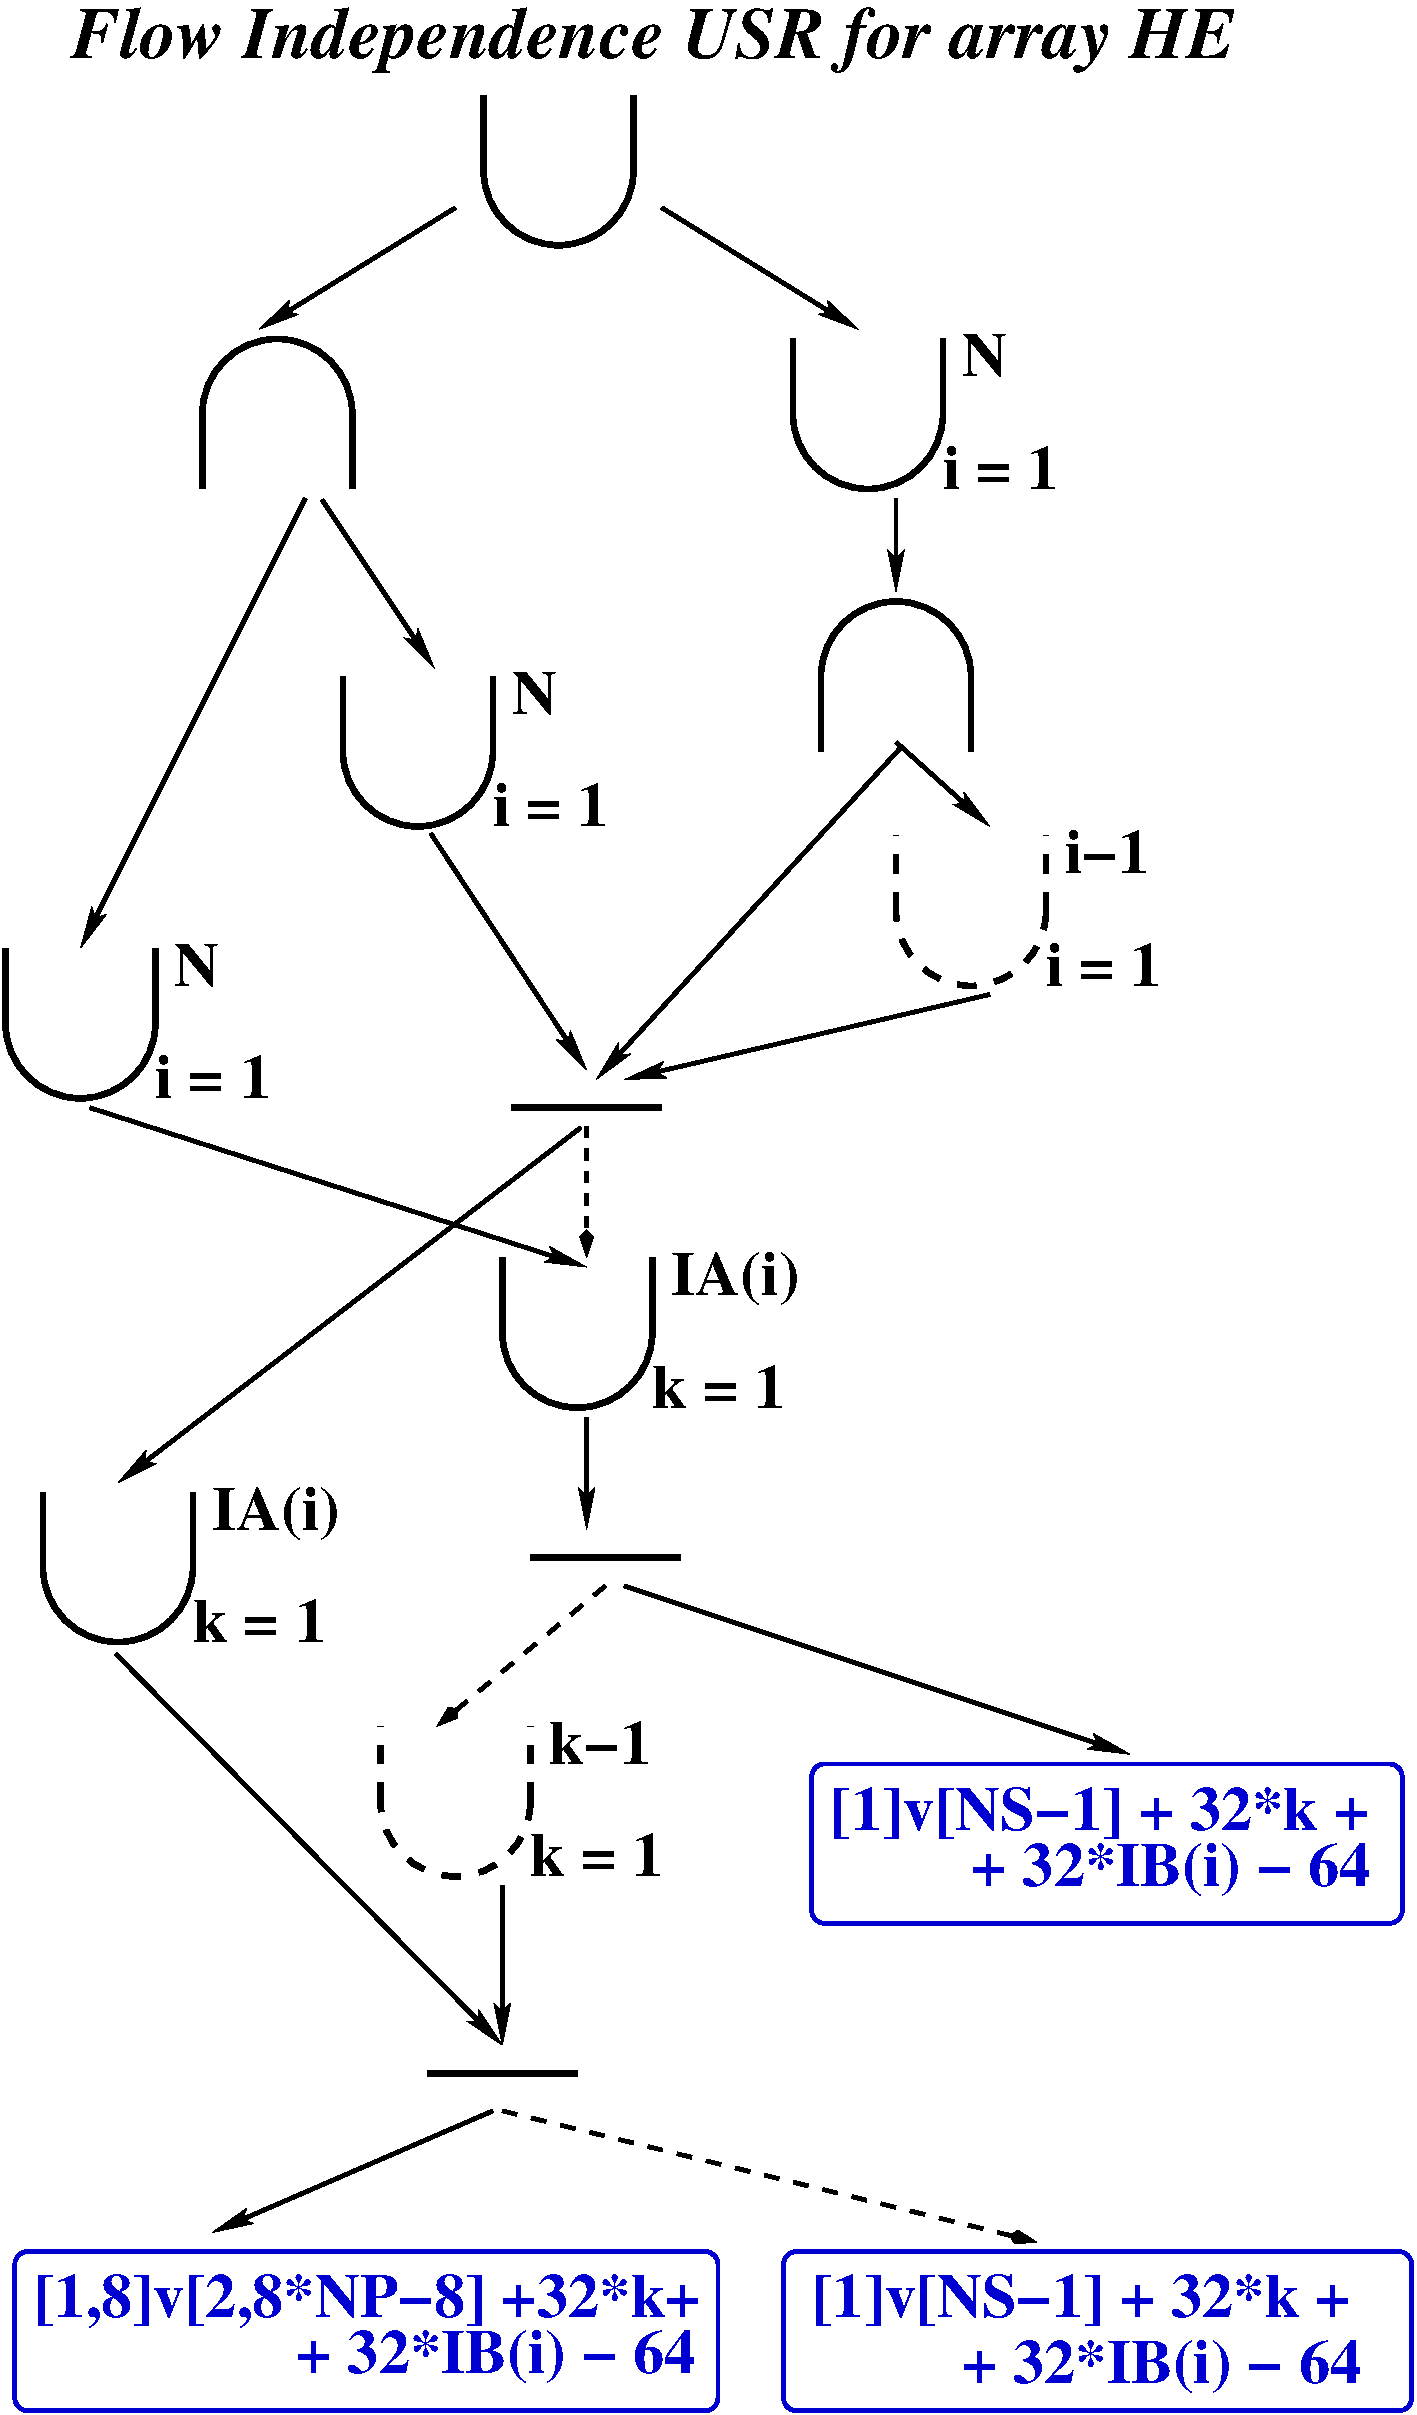
\includegraphics[scale=0.16]{Figures/SOLVH_DO20_FIGS/NEW/USR_HE_FIND_SOLVH}\\
(a)
\end{minipage}
\begin{minipage}{0.5\columnwidth}
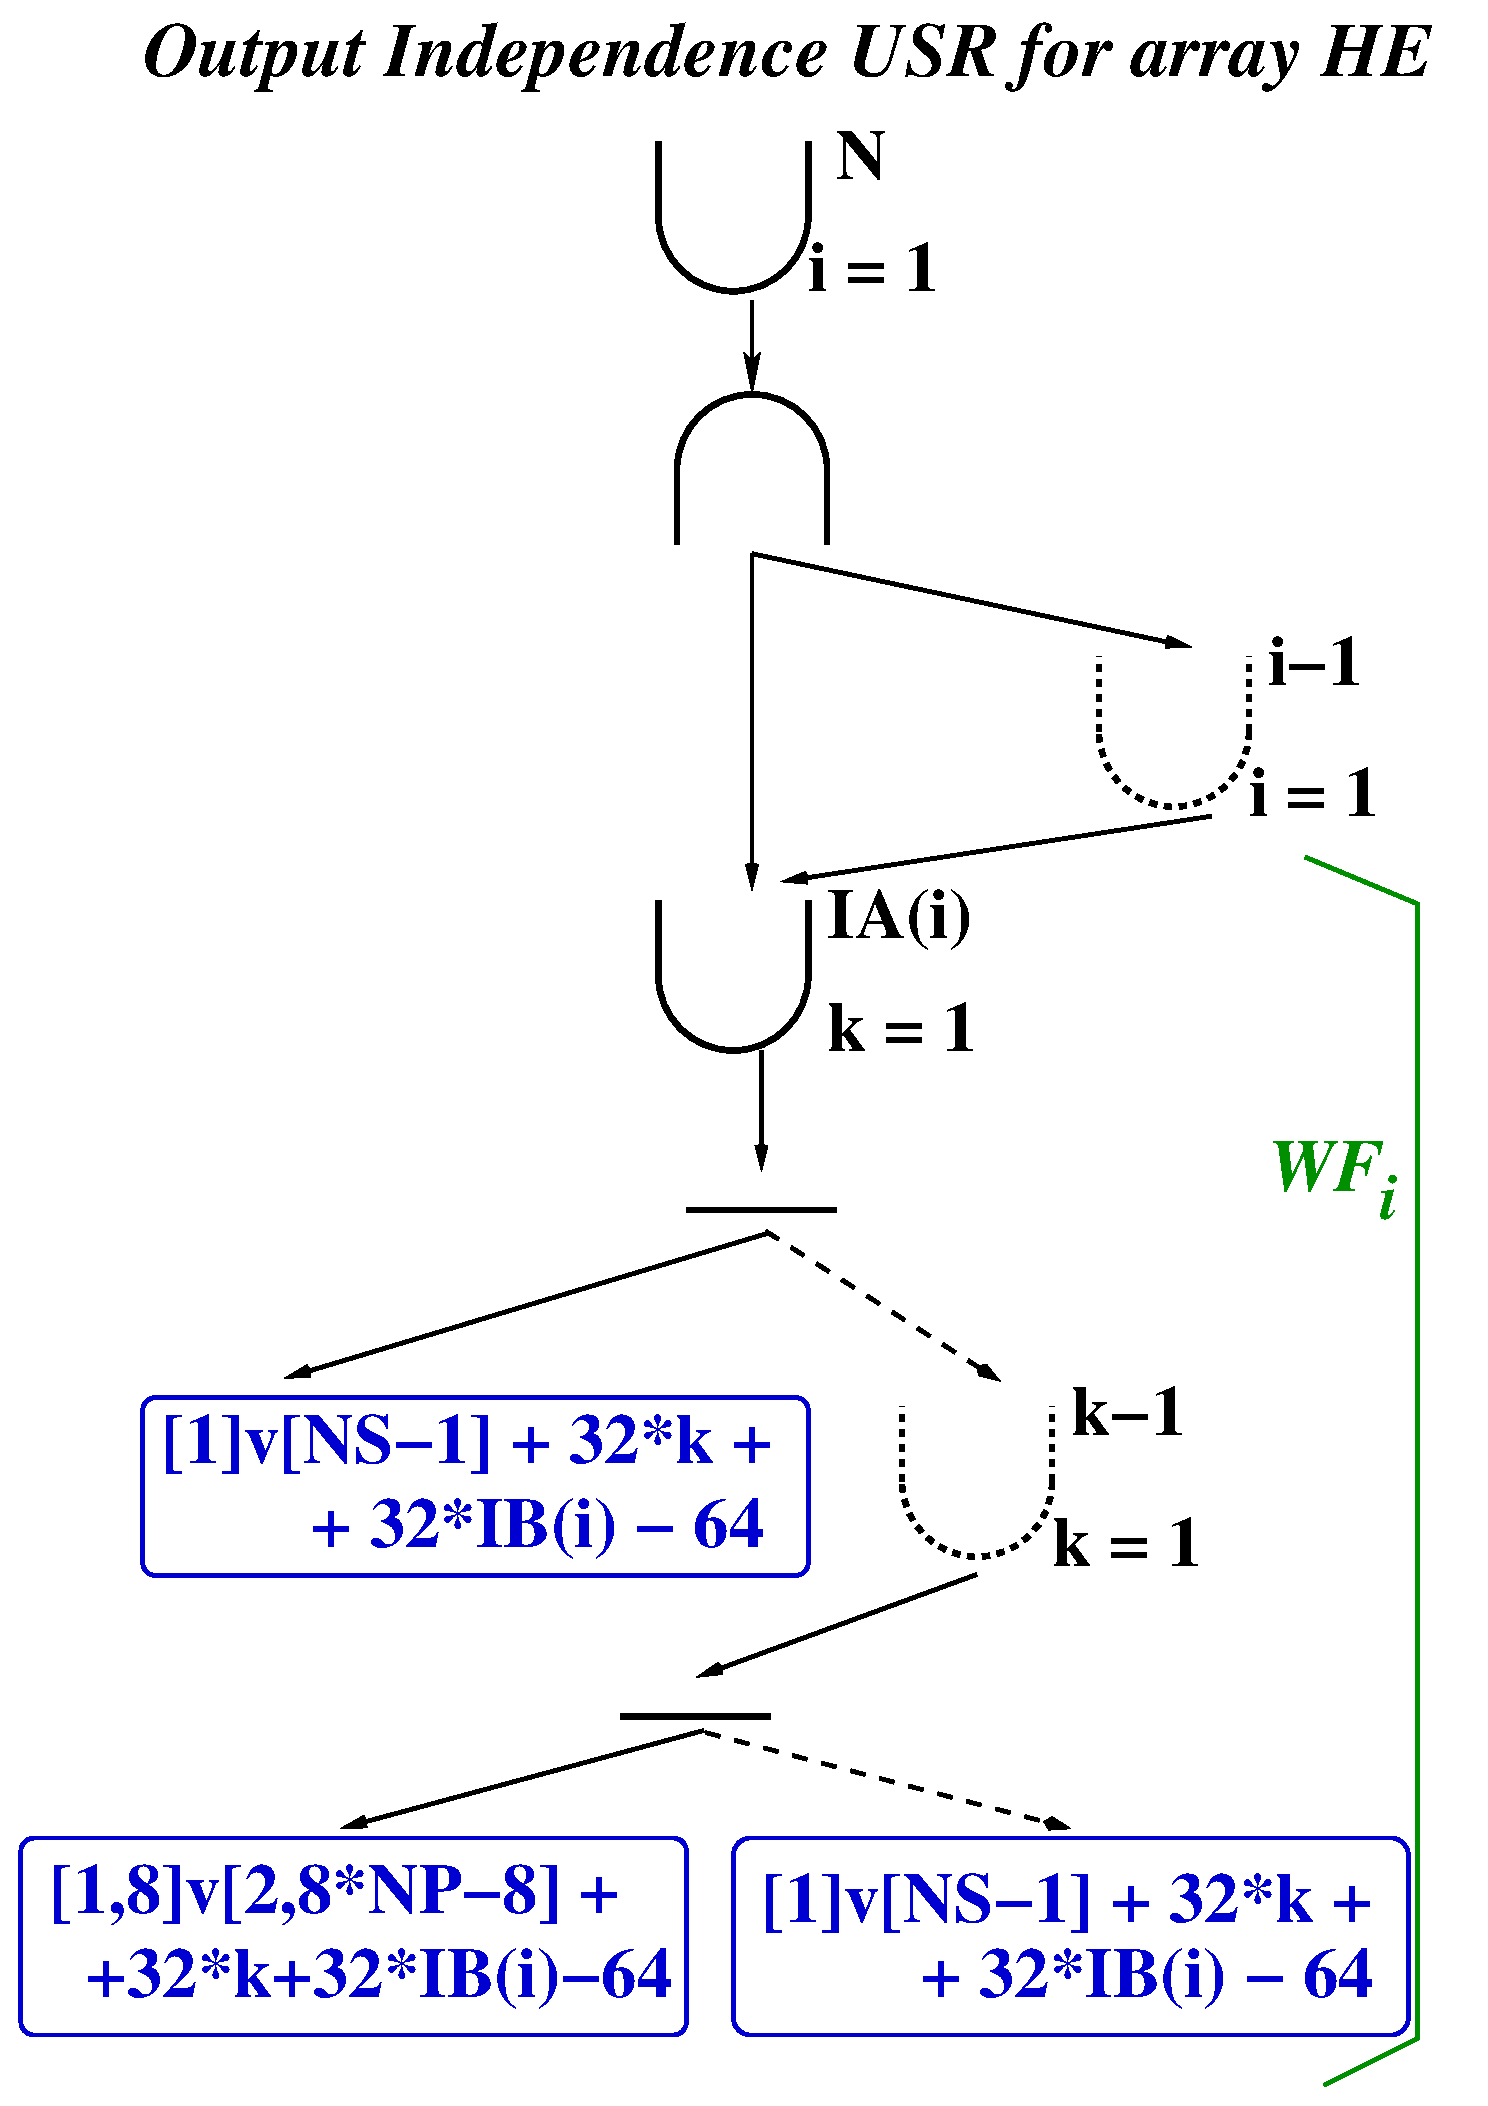
\includegraphics[scale=0.115]{Figures/SOLVH_DO20_FIGS/NEW/USR_HE_OIND_SOLVH}\\
(b)

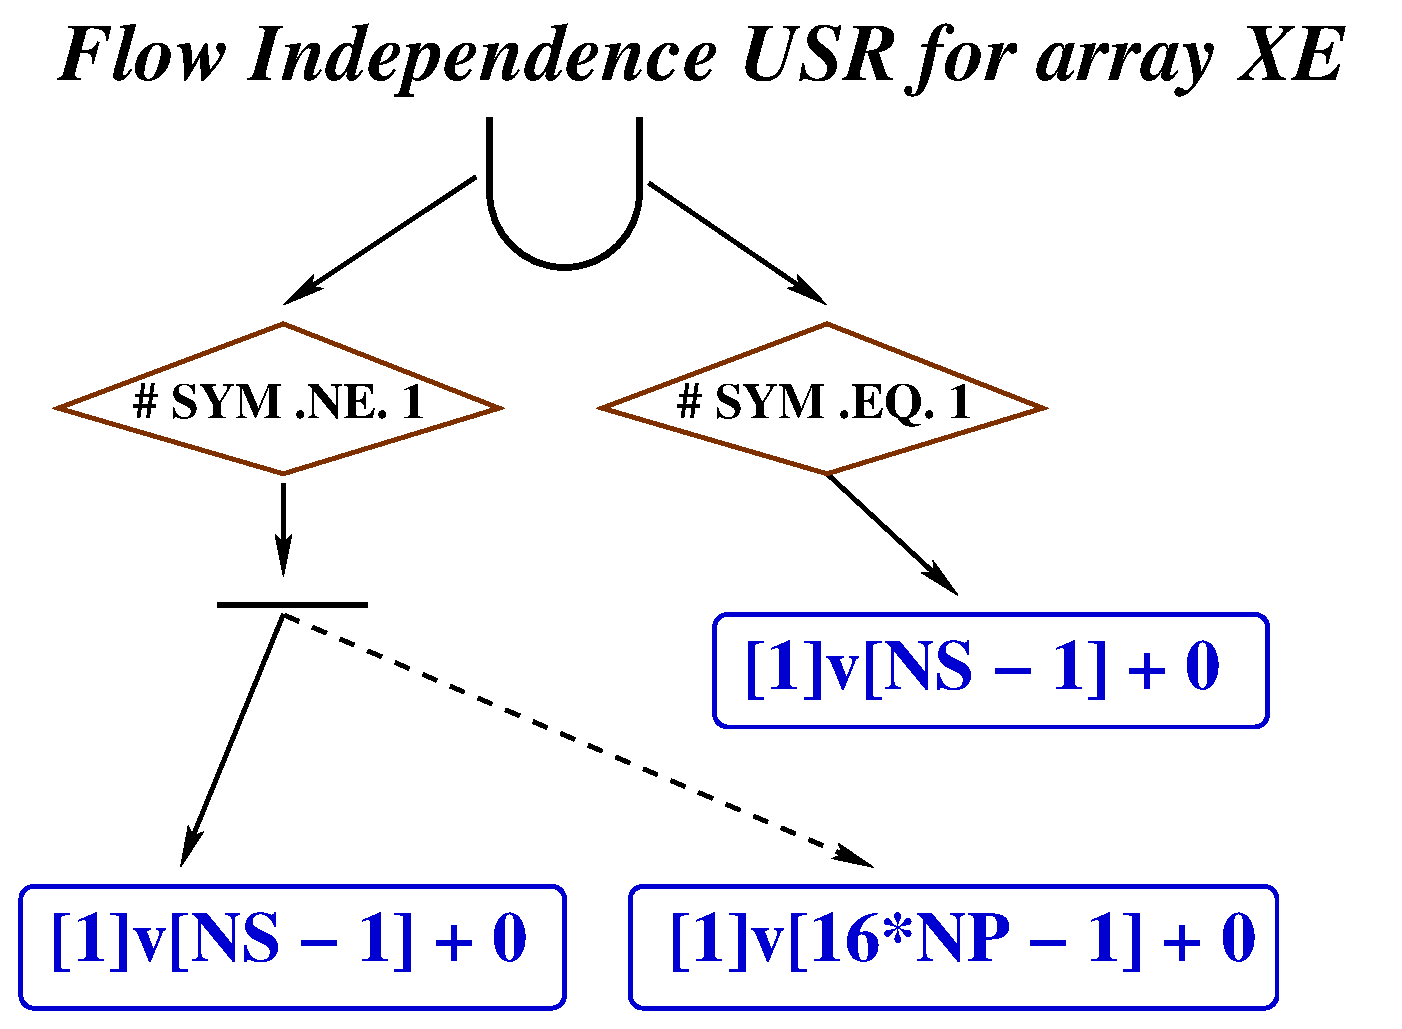
\includegraphics[scale=0.115]{Figures/SOLVH_DO20_FIGS/NEW/USR_XE_FIND_SOLVH}\\
(c)
\end{minipage}
\hrule
\caption{Flow/Output Independence USRs for {\tt HE}, {\tt XE} in Figure~\ref{fig:SolvhDO20Code}.
Corresponding {\sc f/o-ind} Predicates are: (c)~{\tt SYM.NE.1$\wedge$NS$\leq$16*NP},
(a)~{\tt 8*NP<NS+6}, 
(b)~$\wedge_{i=1}^{N-1}${\tt NS$\leq$32*(IB(i+1)-IA(i)-IB(i)+1)}.
Dotted line points to the subtracted part; dotted $\cup_{i=1}^{i-1}$ 
denotes partial recurrence under a fresh variable that ranges from $1$ to $i-1$.}
\label{fig:SOLVH20USR}
\end{figure}


{\sc usr}'s {\em internal nodes} represent operations that cannot be accurately 
expressed in the {\sc lmad} domain: (i) irreducible set operations, 
such as union, intersection, subtraction ($\cup$, $\cap$, $-$), 
or (ii) control flow: gates predicating summary's existence, 
call sites across which summaries cannot be translated, 
or total ($\cup_{i=1}^{N}$) and partial ($\cup_{k=1}^{i-1}$) recurrences %/loops
that fail exact aggregation.
%loops that fail exact aggregation. %in the {\sc lmad} domain.
%
For example, with the {\sc usr} in Figure~\ref{fig:XE_FIND}, the set subtraction
between {\sc lmad}s $[1]\vee[{\tt NS}-1]+0$ and  $[1]\vee[16*{\tt NP}-1]+0$
cannot be represented in the symbolic {\sc lmad} domain, hence a subtraction
{\sc usr} node ($-$) was introduced. 
%
Moreover, the resulting (subtraction) set
is part of the result {\it iff} gate ${\tt SYM .NE.} 1$ holds, etc.
We note that resorting to conservative approximation 
%(to keep the result inside the {\sc lmad} domain) 
instead of introducing the subtraction node, would {\em miss} the 
condition under which the loop is provably {\em independent}. 
%
Similar arguments can be made for the {\sc usr}s in 
Figures~\ref{fig:HE_FIND}~and~\ref{fig:XE_FIND}.
%e.g., conservative approximation of the bottom subtraction node of
%array {\tt HE}'s {\sc find-usr} would miss the relevant 
%independence condition.

\subsection{Loop Independence as USR Equations (IND-USR)}

Having summarized accesses at loop level, answering loop independence 
reduces to establishing the satisfiability of an independence equation
in the {\sc usr} domain.
%
Denoting by $(WF_i,RO_i,RW_i)$ the per-iteration write-first, read-only and 
read-write summaries of array $X$ in loop $L$, where $L$'s iterations range 
from $1$ to $N$, the output independence of array $X$ in $L$ is represented 
via equation: 
\begin{equation}\label{OIEq}
\{ \cup_{i=1}^{N}(WF_i \cap (\cup_{k=1}^{i-1}WF_k))\} = \emptyset
\end{equation}
Equation~\ref{OIEq} states that if for any $i$, the write-first set of iteration $i$
does not overlap with the write-first set of any iteration preceding $i$, then
no two different iterations write the same location, hence no cross-iteration
dependency exists. We name the left-hand side of equation~\ref{OIEq} the 
output-independence {\sc usr} ({\sc oind-usr}) of $X$ in $L$.

Similarly, flow-anti independence is established via equation: 

\begin{equation} \label{FIEq} 
\begin{array}{l  r }
\{(\cup_{i=1}^{N}WF_i) \cap (\cup_{i=1}^{N}RO_i)\} \cup 
\{(\cup_{i=1}^{N}WF_i) \cap (\cup_{i=1}^{N}RW_i)\} \cup  & \\
\{(\cup_{i=1}^{N}RO_i) \cap (\cup_{i=1}^{N}RW_i)\} \cup 
\{ \cup_{i=1}^{N}(RW_i \cap (\cup_{k=1}^{i-1}RW_k))\}  = \emptyset &
\end{array}
\end{equation}
where we denote the left-hand side via {\sc find-usr}. 
%
Figure\ref{fig:SOLVH20USR} depicts the independence {\sc usr}s of our
running example, where {\sc lmad} leafs were seen as intervals in 
Section~\ref{subsec:IntroCodeEg}.

When the independence {\sc usr} ({\sc ind-usr}) is definitely empty or non-empty
the loop can be classified statically as independent or dependent, respectively.
%
In numerous cases, however, independence is either statically undecidable, 
for example because certain variables are input dependent, or too complex
to analyze with the current compiler infrastructure.
In principle, a solution would be to directly evaluate {\sc ind-usr} 
at run-time, and to implement conditional loop parallelization based 
on the independence result. 

This technique works well in some special instances: (i) when {\sc ind-usr}
has $O(1)$ runtime complexity, as with the {\sc usr} in Figure~\ref{fig:XE_FIND},
or (ii) when its evaluation is amortized over many executions of the 
loop, i.e., {\sc usr} evaluation has been safely hoisted outside at 
least one outer loop.
In the general case,  however, we have found that runtime {\sc usr} evaluation 
generates very high overhead, when compared with our technique.



%%%%%%%%%%%%%%%%%%%%%%%%%%%%%%%%%%%%%%%%%%%%%
%%% FACTORIZATION: PREDICATE CONSTRUCTION %%%
%%%%%%%%%%%%%%%%%%%%%%%%%%%%%%%%%%%%%%%%%%%%%



%% Acknowledgments
%\begin{acks}
%The authors would like to thank Dr. Maura Turolla of Telecom
%Italia for providing specifications about the application scenario.
%\end{acks}

% Bibliography
\bibliographystyle{ACM-Reference-Format-Journals}
\bibliography{HybPredAn.bib}
                             % Sample .bib file with references that match those in
                             % the 'Specifications Document (V1.5)' as well containing
                             % 'legacy' bibs and bibs with 'alternate codings'.
                             % Gerry Murray - March 2012

% History dates
%\received{February 2007}{March 2009}{June 2009}
\end{document}
